
\chapter{Introduction}

This thesis presents a systematic theoretical study of the interaction and interplay between a new class of materials named Topological Insulators (TIs) and superconductors. It consists of five chapters. The first chapter contains a brief introduction to TIs and superconductors. In addition, it describes basic concepts and notations used later in the bulk of the thesis. These include the topological surface states of a TI, the spin texture of the TI surface, phenomenological description of a superconductor coupled to a TI, exotic superconductors, and a Josephson junction structure on a TI surface. The second chapter presents a study of the interaction between metal and TI, and electron scattering at the M-TI interface. This chapter provides insight into understanding the effect of spin-orbit interactions on incoming arbitrarily spin-polarized electrons. The third chapter is a microscopic study of a heterostructure of a superconductor with a TI. The motivation is to understand the effect of a TI on an $s-$wave superconductor. The fourth chapter examines Josephson junctions on a TI surface and delves into new aspects of the energy spectra in regimes not studied before. 
%
%The fourth chapter describes an investigation on the newly proposed scheme to engineer a gapless Weyl superconductor through layering of superconductors and TI. Each of the chapters has an introduction section that outlines how the focused study plays a role in the larger scheme of the thesis. It will also give an overview of the chapter and what parts have been published. 
Each chapter beyond Chapter 1 represents an original work published in Physical Review B. 

\section{Topological Insulators}
The field of condensed matter physics has a history of understanding phases of matter that have been condensed. Where the early focus was on solids and liquids, the field has transitioned into studying a rich variety of novel phases that are much more complex. A result of the exploration of many of these novel phases, the concept of order arose, allowing, not only the ability to categorize these phases by recognizing the type of order the system had but the order is usually associated with symmetries of the system. This idea is clearly seen in the phase transition of liquid atoms with rotational and translational symmetry into a crystal with discrete symmetries (e.g. translational, discrete rotational, inversion, etc.). An extension to this would be a paramagnet transitioning into a ferromagnet, thus breaking time-reversal symmetry. While this study of symmetry breaking is at the heart of condensed matter and allows for a deeper understanding, it is not the full story. 

In 1980 Klaus von Klitzing et al performed an experiment measuring the Hall conductance of semiconductor heterostructures in a strong magnetic field\cite{klitzing_new_1980}. What they found in the experiment was that the measured Hall conductance came in exact quantized fundamental units of $e^2/h$,
\begin{equation}
\sigma = \nu \frac{e^2}{h},
\end{equation} 
where $\nu$ is an integer value. 
The significance of this result was not only in the quantized nature of the Hall conductance, but something a bit deeper. This integer quantum Hall effect was special because this result could not be described through the usual symmetry breaking language. In the heterostructure used in the experiment, the internal ``bulk" of the system is effectively a two dimensional electron gas exposed to a strong magnetic field. The strong magnetic field puts the electrons in a cyclotron orbit and forces the electrons into discrete energy levels, the Landau levels. This effect is rather similar to a harmonic oscillator where an electron is in a spatially quadratic electric potential well ($V(x)\propto x^2$). These separated energy levels allows for the system to be an insulator when the Fermi energy is placed within the gap between two separate energy levels. While this system is in an insulating state,the edge is still a host to electronic states that propagate in a chiral manner. This discrepancy between the ability to describe bulk of the material and its edge is the issue at hand. 

The quantum Hall effect (QHE) is actually a topological phase of matter, with its energy bands described by topological invariants known as Chern numbers.
%, meaning it has topological order. Systems with topological order have long-range entanglement and a ground state degeneracy that cannot be lifted by any local perturbation. 
An integer QH phase protected from being deformed into a phase with different topology in the same way a donut (torus) is protected from being deformed into a sphere. The only time such a change is possible is through a phase transition where the gap in the energy spectrum closes in a critical fashion. 
More discussions on topological phases of matter can be found in literature.
%Many discussions on topological order can be found in many literature and any continued discussion about topological order in farther depth would not be appropriate, for this thesis does not represent any study of topological order in this form. 

\begin{figure}
\center
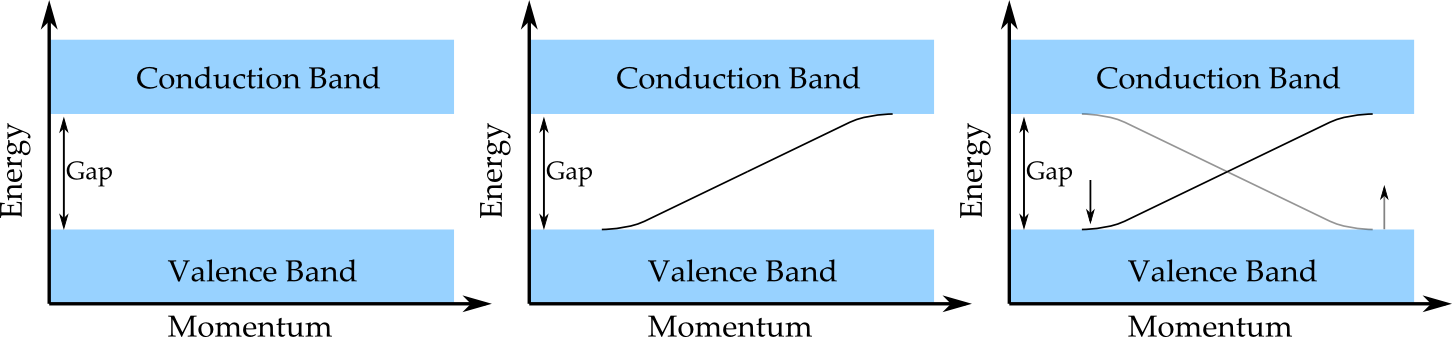
\includegraphics[width=\textwidth]{include/bands2.png}
\caption{(a) Energy spectrum of a trivial band insulator where two bands, conduction and valence, are separated by an energy gap. 
(b)  Energy spectrum of a quantum Hall state. The gap now has one chiral edge state connecting the valence band to the conduction band.  
(c)  Energy spectrum of a 2D TI (QSH). The gap now has one pair of chiral edge states connecting the valence band to the conduction band.  One line is for the spin up state and the other is for the spin down state. This essentially mimics two copies of the quantum Hall state for each spin.
}\label{insulators}
\end{figure}

We use the QHE as a lead-in for the topological insulator. 
%Though the topological insulator is a slight misnomer because of the lack of topological order (i.e. long-range entanglement), we will shortly see where the topology plays a role in it. 
By taking the QHE, we can extend it in the following way. The QHE is a gapped system with chiral edge states that depend on the applied magnetic field (see Fig. \ref{insulators}). The chirality of the edge states depend on the direction of the magnetic field, i.e. positive (negative) chiral motion of the electrons for positive (negative) out of plane magnetic field. If a system were to have both positive and negative magnetic fields simultaneously for two different species of electrons, we would see the electrons follow the two chiral motions simultaneously depending on their species. The two different species of electrons are, of course, spin-up and spin-down electrons which couple to the two magnetic fields. This system is a prototype of the quantum spin Hall effect. Kane and Mele first proposed the QSH to exist in graphene with spin-orbit coupling \cite{kane_quantum_2005}. Shortly afterwards, Bernevig, Hughes, and Zhang proposed a realistic experimental setup to host the QSH effect \cite{bernevig_quantum_2006}. Their proposal, which was verified successfully in an experiment by Koenig's group \cite{konig_quantum_2007}, exploited the spin-orbit coupling and band inversion in a HgTe-CdTe-HgTe heterostructure to create pairs of counter-propogating edge states, which are related to each other by time reversal symmetry. The QSH insulator is a 2D topological insulator. An effective Hamiltonian for the edge state can be written as 
\begin{equation}
H=\hbar v_F \sigma_x k_y,
\end{equation}
where the basis is for spin up and spin down and the resulting eigen energies are $E=\pm \hbar v_F k_y$. $v_F$ is the Fermi velocity. This is a massless Dirac Hamiltonian and the spectrum forms a Dirac crossing. 
 
The existence of a surface state can be seen in the following manner. If a topological insulator has a parameter that can be tuned to transition from topologically non-trivial to trivial, the gap of the insulator must close. When a TI is interfaced with a trivial insulator, such as the vacuum, the parameter effectively causes the gap to close at the interface, which gives rise to the gapless surface state.

In principle, by stacking sheets of the 2D TIs and forming a 3D structure, this would be a ``weak" topological insulator. The other extension of the TI from 2D to 3D  is a ``strong" topological insulator. Here, there is also an insulating 3D bulk and the 2D surfaces interfacing the vacuum are similar to the edge state of the 2D TI in their linear dispersing behavior, but they allow momentum to be in any in-plane direction, $\vec{k}=(k_x,k_y)=(k \cos(\theta),k \sin(\theta))$. The effective low-energy Hamiltonian for these surface states is
\begin{equation}
H=\hbar v_F (\sigma_x k_y - \sigma_y k_x).
\end{equation}
The energies and their respective eigenvectors
\begin{equation}
E=\pm \hbar v_F |\vec{k}|\quad
\ket{\psi_{\bf{k}}}=\frac{1}{\sqrt{2}}\left(\pm i e^{-i \theta}\ket{\uparrow}+\ket{\downarrow}\right)
\end{equation}
 where $|\vec{k}|=\sqrt{k_x^2+k_y^2}$ and $\ket{\uparrow}(\ket{\downarrow})$ is the spin up (down) state.
 
 We plot the energy dispersion as a function of $k_x$ and $k_y$ to find a Dirac cone in Fig. \ref{cone}. Any cut taken for some value of $E\neq0$ produces a circle of states. The eigenstates are always equal superpositions of spin up and down, meaning the spinor is pointing in the x-y plane. The exact direction is dictated by the phase ($ie^{i \theta}$). The spin is pointing at a $\pi/2$ angle from the momentum direction at angle $\theta$, due to the extra $i$.

\begin{figure}[h]
\center
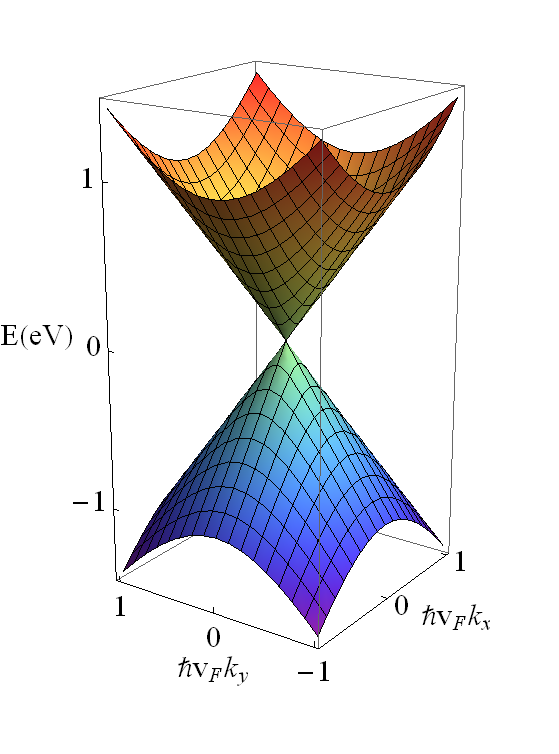
\includegraphics[width=.6\textwidth]{include/cone.png}
\caption{Dirac cone dispersion. Energy as a function of momentum, $k_x$ and $k_y$.
}\label{cone}
\end{figure}
 
 If we look closely at the spin-momentum relationship we see that it is not possible to have arbitrary spin and momentum for an electron on the TI surface. Every direction of momentum is locked to one direction of spin and vice versa. 
 %This can be seen as a broken symmetry of the surface electrons where they no longer have arbitrary spin and momentum. 
 This surface is very different from a normal metal where spin is arbitrary for any momentum and also different from a ferromagnet where the spin of an electron is fixed but can have arbitrary momentum. This coupling along with the relativistic energy dispersion is unique and provides a playground for many exotic properties. These include Majorana fermions\cite{fu_superconducting_2008,hasan_colloquium:_2010,linder_unconventional_2010,qi_topological_2011}, barrier transmission \cite{seo_transmission_2010}, spin-currents \cite{yazyev_spin_2010,burkov_spin_2010}, Aharanov-Bohm oscillations \cite{peng_aharonov-bohm_2010}, Shubnikov-de Haas oscillations \cite{analytis_bulk_2010}, Landau level quantization \cite{cheng_landau_2010}, massive relativistic Dirac fermions \cite{liu_magnetic_2009, lu_massive_2010}, and exciton condensation \cite{seradjeh_exciton_2009}.
 
In 2008, Hassan's group found a 3D TI in the form of Bi$_{.9}$Sb$_{.1}$ by way of ARPES measurements\cite{hsieh_topological_2008}. They found a linear dispersion, Dirac crossing, on the surface and while the bulk has a gapped energy spectrum. This experiment was motivated by several theoretical predictions\cite{fu_topological_2007,fu_topological_2007-1} to find topological insulators in such a 3D binary compound due to the spin-orbit coupling in the material. This led to the discovery of other TIs; Bi$_2$Se$_3$, Bi$_2$Te$_3$, Sb$_2$Te$_3$; as well as finding topological properties of pure Sb\cite{hsieh_tunable_2009,hsieh_observation_2009,hsieh_observation_2009-1,roushan_topological_2009,seo_transmission_2010}. Since the discovery in 2008, there has been an explosion in research on topological insulators in ArXiv.org, where in years 2009, 2010, 2011, 2012 there were 100, 235, 362, 421 papers on topological insulators, respectively. 
 
This concludes our basic description of the TI. We showed how a 2D TI was produced using two copies of a QH system with opposite simultaneous magnetic fields. We then extended the idea of a 2D TI to 3D ``weak" and ``strong" TIs. We then examined the surface states to understand the relationship between the spin and momentum as well as potential implications and applications.  
 
 % A simple exercise to see the insulator-surface state behavior described, we present a simplified version of the accepted model Hamiltonian for bulk Bi$_2$Se$_3$:
 % \begin{equation}
% H= (M_0+M k^2)\tau_z + A(\sigma_x k_y - \sigma_y k_x)\tau_x +B \sigma_z k_z \tau_y,
% \end{equation}
 % where $\sigma (\tau)$ represent spin (orbital) basis, $A,B,M,M0$ represent physical parameters of the system. This Hamiltonian can be diagonalized to find energy eigenvalues of 
  % \begin{equation}
% E= \pm\sqrt{(M_0+M k^2)^2 + A^2(k_x^2 + k_y^2) +B^2 k_z^2}.
% \end{equation}
 % A three step inspection can show how two critical ingredients are needed for this to be a topological insulator. By setting $A=B=0$ and having $M_0>0$, we see that we have a trivial insulator with a band-gap of $2 M_0$. By adjusting this gap parameter to negative values, $M_0<0$, we see the valence and conduction bands intersect at $E=0$. To transition this to an insulator we can set $A \neq 0$ and $B \neq 0$, in effect turning on spin orbit coupling. We now see a gap arise and through additional steps we find that this setup is host to surface states. To find these surface states we set the form of the wave functions to be 
   % \begin{equation}
% \psi \propto e^{\Lambda z}
% \end{equation}
% as an ansatz from an assumption that $H(x,y,z=0,L)=0$ and that the surface states reside on the boundaries decay into the bulk. We also make the substitution of $k_z \rightarrow -i \partial_z$. The Hamiltonian is now in the form
  % \begin{equation}
% H= (M_0+M (k_x^2+k_x^2-\Lambda^2))\tau_z + A(\sigma_x k_y - \sigma_y k_x)\tau_x +B \sigma_z (-i)\Lambda \tau_y.
% \end{equation}
% To verify the existence of a Dirac crossing at zero energy, we diagonalize the Hamiltonian and set $k_x=k_y=E=0$ and find that there exists values for $\Lambda$:
  % \begin{equation}
% \Lambda=\pm \frac{B\pm \sqrt{B^2+4M M_0}}{2M}
% \end{equation}
% illustrating that surface states do indeed exist. 


\section{Superconductivity}

\subsection{Measurement}
Superconductivity was discovered by Heike Kamerlingh Onnes in 1911.
%is usually the first item that's discussed when the topic of superconductivity is brought up. In the discovery, Onnes 
He found that the resistance of mercury drops to zero as the temperature is lowered below 4.2K, a signature of perfect conduction. An immediate question arises, if using a typical voltmeter, as used in physics labs, and Ohm's law, $V=IR$, how can resistance or voltage be measured if they should both be zero? The answer is by using a four point probe. As seen in the diagram in Fig. \ref{measures}, the probe has four point of contact on the material. Two of the connections (1,4) have a constant, controllable current flowing through them. The other two connections (2,3), then probe the sample and measure the voltage drop. The voltage measurement device has a high impedance to minimize any flow from the sample into it. The resulting voltage drop, V, and driving current, I, then give the resistance, $R=V/I$, which along with temperature results in a temperature dependent resistance. An example measurement of Cu$_{.2}$Bi$_2$Se$_3$, a new superconducting material based on the topological insulator Bi$_2$Se$_3$, is shown in Fig. \ref{measures}. The plot shows a clear resistance drop at 3.5 Kelvin, the signature of superconductivity. 
\begin{figure}
\center
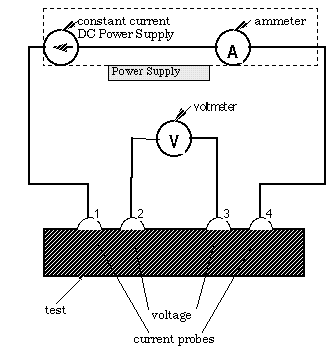
\includegraphics[width=.45 \textwidth]{include/fourprobe.png}
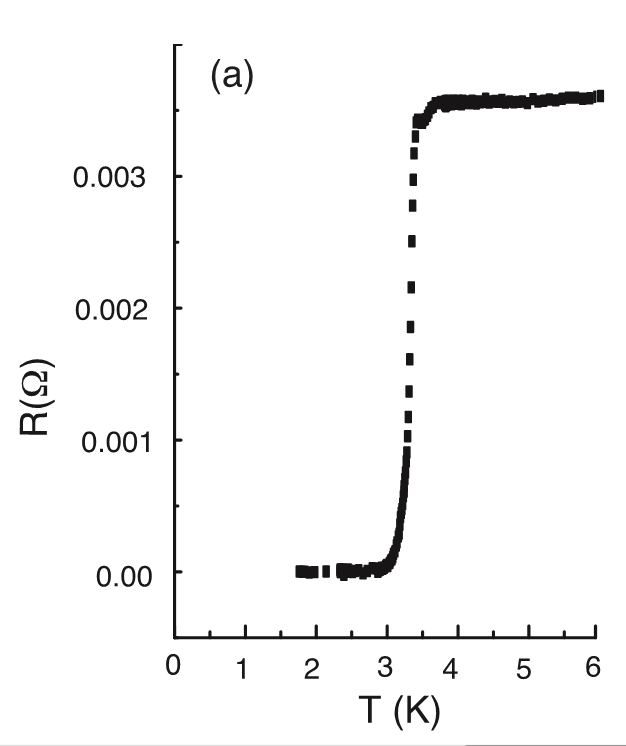
\includegraphics[width=.45 \textwidth]{include/resistance.png}
\caption{(left) Four probe measurement device. Probes 1 and 4 are used to flow a current across a sample while probes 2 and 3 measure the voltage drop across the sample where the current is flowing. (right) Resistance ($\Omega$) vs Temperature (Kelvin) experiment on Cu$_{.2}$Bi$_2$Se$_3$ from arXiv:1111.5805. The drop in resistance is a signature of superconductivity. \label{measures}
}
\end{figure}
\clearpage
\subsection{BCS and Bogoliubov Theory}
Bardeen, Cooper, and Schreiffer (BCS) came up with a theory to explain the mechanism behind superconductivity. We start with the Hamiltonian that represents a free electron system with two-body electron interactions,
\begin{equation}
H=\sum_{\bf{k},\sigma} (\epsilon_{\bf{k}}-\mu)
c^{\dagger}_{\bf{k}\sigma}
c_{\bf{k}\sigma}+
\sum_{\bf{k},\bf{l'}}
V_{\bf{k},\bf{k'}}\, 
c^{\dagger}_{\bf{k}\uparrow}
c^{\dagger}_{-\bf{k}\downarrow} 
c^{}_{-\bf{k'}\uparrow}
c^{}_{\bf{k'}\downarrow}
\end{equation}
where $c^{\dagger}_{\bf{k}\sigma}$ ($c_{\bf{k}\sigma}$) is the electron creation (annihilation) operator, the summations are over spin ($\sigma$)and momentum ($\bf{k},\bf{k'}$), $\epsilon_{\bf{k}}$ is the free electron energy, $V_{\bf{k,k'}}$ is the electron-electron interaction potential. The commutation relations for the fermion creation and annihilation operators are
\begin{equation}
\{c^{\dagger}_{\bf{k}\sigma},c_{\bf{k'}\sigma'}\}_+=\delta_{\bf{k},\bf{k'}}\delta_{\sigma \sigma'}
\end{equation}
\begin{equation}
\{c^{\dagger}_{\bf{k}\sigma},c^{\dagger}_{\bf{k'}\sigma'}\}_+=\{c_{\bf{k}\sigma},c_{\bf{k'}\sigma'}\}_+=0.
\end{equation}

In usual electron systems, the Coulomb interaction between electrons is repulsive, but the effective interaction can become attractive. 
% scattering potential, $V_{\bf{k k'}}$, usually positive, represents repulsive interactions. But as the temperature is lowered, what BCS explained was that the repulsive interaction was no longer the dominant interaction. Instead, what occurs at zero temperature is the following. 
As an electron passes through a lattice of low-mobility nuclei, they actually cause the nuclei to shift causing a phonon interaction with electron. This phonon interaction can be strong enough to effectively attract, $V_{\bf{k k'}}<0$, two electrons with opposite momenta($\bf{k},-\bf{k}$). From the Pauli exclusion principle, we seek a bound pair of electrons with zero total momentum and antisymmetric wave functions known as a Cooper pair. When the electrons pair, they form a condensate of the bosons, which supports superflow that is responsible for the lack of resistance. 
The electrons near the Fermi energy are most susceptible to pairing, usually when they are within some Debye energy cutoff, $\hbar \omega_D$. One way to describe the superconductor is through a condensate wave function or more precisely the superconducting order parameter, $\Delta(\bf{x})$, or $\Delta_{\bf{k}}$. This function is found by a mean field approach to the pairing potential, $V_{\bf{k k'}}$, through the gap equation
\begin{equation}
\Delta_{\bf{k}}=\sum_{\bf{k'}}
V_{\bf{k k'}}\,
c^{}_{-\bf{k'}\uparrow}
c^{}_{\bf{k'}\downarrow}
\end{equation}
reducing the Hamiltonian down to 
\begin{equation}
H=\sum_{\bf{k},\sigma} (\epsilon_{\bf{k}}-\mu)
c^{\dagger}_{\bf{k}\sigma}
c_{\bf{k}\sigma}+
\sum_{\bf{k}}
\Delta_{\bf{k}}\, 
c^{\dagger}_{\bf{k}\uparrow}
c^{\dagger}_{-\bf{k}\downarrow} +
h.c.
\end{equation}
To diagonalize this Hamiltonian we change the basis, where rather than restricting ourselves to operators of electrons, we use the Bogoliubov-de Gennes (BdG) transformation to introduce the operators on quasiparticle excitations of particles and holes. This is done through
\begin{equation}
c_{\bf{k}\sigma} = \sum_n u_{n \bf{k} \sigma} \gamma_{n\bf{k}}+v^\ast_{n \bf{k} \sigma} \gamma^\dagger_{n\bf{k}},\quad
c_{\bf{k}\sigma}^\dagger = \sum_n u_{n \bf{k} \sigma}^\ast \gamma_{n\bf{k}}^\dagger+v_{n \bf{k} \sigma} \gamma_{n\bf{k}}
\end{equation}
where the quasiparticle operators fulfill the anti-commutation relations,
\begin{equation}
\{\gamma^\dagger_{\bf{k}\sigma},\gamma_{\bf{k'}\sigma'}\}=\delta_{\bf{kk'}}\delta_{\sigma\sigma'} ,\qquad 
\{\gamma_{\bf{k}\sigma},\gamma_{\bf{k'}\sigma'}\}=
\{\gamma^\dagger_{\bf{k}\sigma},\gamma^\dagger_{\bf{k'}\sigma'}\}=0
\end{equation}
and allow us to diagonalize the Hamiltonian as
\begin{equation}
H=E_0+\sum_{\bf{k},\sigma} E_{\bf{k}}
\gamma^{\dagger}_{\bf{k}\sigma}
\gamma_{\bf{k}\sigma}.
\end{equation}
The quasiparticle (quasihole) wave function is $u_{\bf{k}\sigma}$ ($v_{\bf{k}\sigma}$). Each electron creation/annihilation operator is a superposition of a quasiparticle creation and annihilation operator. The inverse of this transformation,
\begin{equation}
\gamma_{\bf{k}\sigma} = \sum_n u_{n \bf{k} \sigma} c_{n\bf{k}}-v^\ast_{n \bf{k} \sigma} c^\dagger_{n\bf{k}},\quad
\gamma_{\bf{k}\sigma}^\dagger = \sum_n u_{n \bf{k} \sigma}^\ast c_{n\bf{k}}^\dagger-v_{n \bf{k} \sigma} c_{n\bf{k}}
\end{equation}
 leads to each quasiparticle operator being a superposition of the electron creation operator and the hole creation operator. This physical interpretation allow us to see that there is more to the story than just electrons and holes, but electron-like and hole-like quasiparticle excitations.

The form of the BdG Hamiltonian is 
\begin{equation}
H_{B}=\left( \begin{array}{cc}
\epsilon_{\bf{k}}-\mu   &-\hat{\Delta}_{\bf{k}}\, i\sigma_y\\ 
\hat{\Delta}^{\dagger}_{\bf{k}} \, i\sigma_y &  \mu-\epsilon_{\bf{k}}
 \end{array} \right), \label{bdgHH} 
\end{equation}
in the basis of 
\begin{equation}
\psi=\left(
u_{\bf{k}\uparrow},
u_{\bf{k}\downarrow},
v_{\bf{k}\uparrow},
v_{\bf{k}\downarrow}\right)^T.
\end{equation}
The $\hat{\Delta}_{\bf{k}}$ can come in a variety of forms, strictly depending on the pairing symmetry of the superconductor. Generally it can be written as $\Delta_{\bf{k}}=\Delta_0(\bf{k})+\bf{d}(\bf{k})\cdot \bf{\sigma}$, while in the BCS case, we focus on $\Delta_{\bf{k}}=\Delta_0$, a constant value, representing s-wave orbital pairing\cite{mineev_introduction_1999}. This allows us to find the eigen values of the system,
\begin{equation}
E_{\bf{k}}=\pm\sqrt{(\epsilon_{\bf{k}}-\mu)^2 + |\Delta|^2}.
\end{equation}
where the spectrum can be seen in the Fig. \ref{bcsplot}. There is now a finite gap of size $2\Delta_0$ seen centered about 0. The gap is a result of the pairing that occurs in the superconductor. These paired states form the condensate and no low energy excitations can exist within the energy gap in the spectrum. In order to have an excitation out of the condensate, you would need $2\Delta_0$ energy to break the pair. 


\begin{figure}
\center
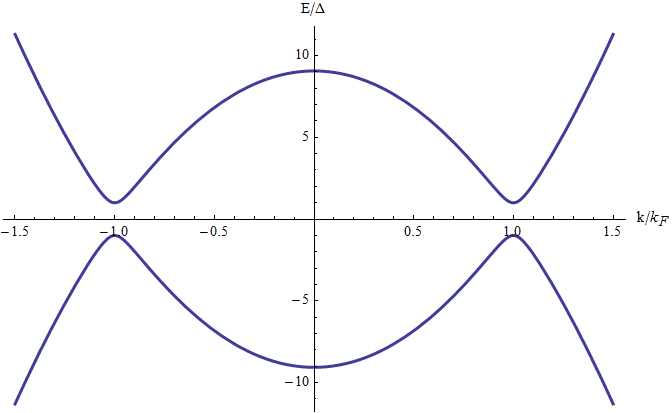
\includegraphics[width=.95 \textwidth]{include/bcsplot.png}
\caption{Energy spectrum for a BCS superconductor with a gap of $2\Delta_0$ and $\mu/\Delta_0=10$.
} \label{bcsplot}
\end{figure}

This concludes the introduction to superconductivity. Here, we reviewed  the BCS theory on superconductivity to describe the mechanism behind the Cooper pairing, and diagonalizing the BCS Hamiltonian using a mean field approximation and the Bogoliubov-de Gennes Transformation to obtain the energy spectrum. These are the building blocks for understanding the discussions on superconductivity in this thesis. 

\section{Topological Superconductors and Superconductor-Topological Insulator Heterostructures}
This section presents two related condensed matter systems that have exotic properties and the motivation for studying them. These are p$_x$+ip$_y$ superconductors and topological insulator-superconductor heterostructures that host Majorana Fermions. These systems have implications in understanding the role of topology in superconducting systems as well as the possibility of topological quantum computation through the Majorana Fermion. This thesis can be viewed as a systematic deeper study of the latter systems beyond phenomenology. 
\subsection{p$_x$+ip$_y$ superconductors}
One kind of a superconductor that has exotic topological behavior is the p$_x$+ip$_y$ superconductor. The symmetry of this paired spin-triplet state is of the form $\hat{\Delta}_k=\Delta_0 (k_x+ik_y) (\sigma_x+i\sigma_y)$. If we apply this form of the pairing into \eqref{bdgHH}, we can diagonalize the BdG Hamiltonian and find eigenvalues of the form

\begin{equation}
E_{\bf{k}}=\pm\sqrt{(\epsilon_{\bf{k}}-\mu)^2 + (\Delta_0|\bf{k}|)^2}.
\end{equation}
This differs from the conventional s-wave eigen energies because the gap term now depends on $\bf{k}$. For values of $\mu>>0$, this doesn't effect the spectrum by any more then a negligible change. The noticeable difference, as described Read and Green\cite{RG}, is when the Fermi energy is reduced to a small value so that $(\epsilon_{\bf{k}}-\mu) \rightarrow -\mu$. The spectrum then evolves into a spectrum for a relativistic Dirac fermion with mass $\mu$ and speed of light $\Delta_0$. We also write the BdG equations in the form of
\begin{eqnarray}
E u=-\mu u + \Delta^\ast i (\partial_x + i \partial_y) v\\
E v=\mu v + \Delta i (\partial_x - i \partial_y) u.
\end{eqnarray}
This is a form of the Dirac equation, and the BdG equations allow for $u=v^\ast$ through charge conjugation symmetry, where at each $\bf{k}$ there is only one excitation mode. This shows that the particles, $u$, are their own anti-particles, $v$. When a Dirac fermion has this property, it is a Majorana Fermion. Now consider a setup for this system where the mass term varies spatially through a a domain wall ($ \mu(x)\propto \text{sign}(x-x_0)$), by tuning the Fermi energy spatially. The requirement for the domain wall is due to the parameter (x) dependent transition from a trivial state superconductor, $\mu<0$ to a non trivial topological superconductor, $\mu>0$. One simple model to do this is by $\mu(x)=\mu \sin(2 \pi x/L)$. We find a spectrum with linear modes in Fig. \ref{pmajorana}. The linear Majorana modes are found to have chiral propagation and reside at the centers of the domain walls. Another way to host a Majorana in a p-wave superconductor is by imposing a vortex through a magnetic field, where at the core of the vortex reside the Majorana modes. 


\begin{figure}[h]
\center
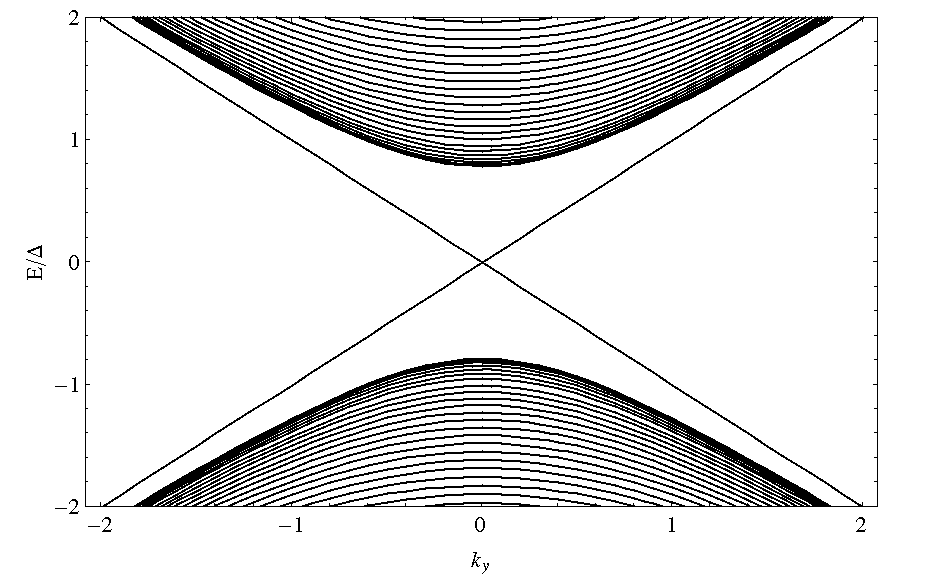
\includegraphics[width=.95 \textwidth]{include/pmajorana.png}
\caption{Energy spectrum for a $p_x\pm ip_y$ superconductor with a chemical potential domain wall, ensuring linearly dispersing Majorana modes.
} \label{pmajorana}
\end{figure}

\subsection{Fu-Kane Superconductor/Topological Insulator Model}
Fu and Kane were the first to describe the effect of a superconductor in close proximity to the surface of a TI\cite{majorana}. The TI has the Hamiltonian in the form of $H=v_F(\sigma_x k_y-\sigma_y k_x) - \mu$, where $k_i$ are the momenta, $\sigma_i$ are the Pauli spin matrices, and $v_F$ is the Fermi velocity. If an $s-$wave superconductor is brought to the surface of the TI, Fu-Kane argued that pairing interaction between electrons will be induced on the surface. 

This interplay between a TI and S presents many possibilities of various physical effects. This system can be seen to mimic a spin-less $p_x\pm ip_y$ superconductor. Also, under certain conditions where there is a domain wall through the superconductor order parameter, $\Delta$ or a magnetic domain wall, it is expected to find a Majorana mode. 

Fu-Kane argued that the form of the pairing term is consistent from the S side to the TI side producing the following BdG Hamiltonian
\begin{equation}
\mathcal{H}(\mathbf{k})=\left(
\begin{array}{cc}
H(\mathbf{k})  &  i\sigma_y  \Delta \\
-i\sigma_y \Delta^*  &   - H^*(-\mathbf{k})
\end{array}
\right)=v_F(\sigma_x k_y-\tau_z\sigma_y k_x) - \tau_z\mu +\tau_y\sigma_y\Delta.
\end{equation}

The spectrum for this system is
\begin{equation}
E=\sqrt{|\Delta|^2 +(v_F |\bf{k}|\pm \mu)^2}.
\end{equation}
This system is very analogous to the p-wave superconductor. If we take the limit $\mu\rightarrow 0$ this dispersion is also relativistic where the mass term is $\Delta$ and the speed of light is $v_F$. The $p_x\pm ip_y$ term is responsible for the resulting Majorana mode. In the superconductor-TI heterostructure, this term is also, as we shall see soon, responsible for producing Majorana modes.
Since the mass term is parameter, it can be tuned to close the gap at one (or an odd number of points) in the spectrum. The mass term in the S-TI system is the gap parameter, $\Delta$. If we allow $\Delta$ to flip sign spatially from a positive value, $|\Delta_0|$, to a negative value, $-|\Delta_0|$, for example through $\Delta(x)=\Delta_0 \tanh( x/L)$, we find a Majorana mode localized at the point where $\Delta(x)=0\, (x=0)$ with a linear dispersion that resembles the spectrum of the p-wave superconductor edge-state in Fig. \ref{pmajorana}. One difference is the TI version is four-fold degenerate (particle/hole) of the $E=0$ mode while the p-wave is two-fold degenerate (particle/hole). Both systems' linear dispersing states are localized at the domain wall, $x=0$. This domain wall can be seen as a Majorana wire in the y-direction.

We've now shown some superconductors with exotic properties. We looked at the p-wave superconductor and how it can be tuned to host Majorana modes along with its relativistic Dirac-like energy dispersion. We also looked at the TI-S heterostructure proposed by Fu and Kane which can be tuned to host Majorana modes. These systems are very analogous to each other and show the potential of engineering topological superconductivity using the hybrid structures of TI and $s-$wave superconductors. The Fu-Kane will be the starting point for latter two thirds of the thesis where we study TI-S structures in greater detail.
